\documentclass{article}
\usepackage{multicol}
\usepackage{graphicx}
\usepackage{makecell}
\usepackage{float}

\title{Cloud Computing - Project Report \\ \small{Totoro Group}}
\author{
    Zahra Omrani \\ z.omrani@studenti.unipi.it \and 
    Paolo Palumbo \\ p.palumbo3@studenti.unipi.it \and
    Ettore Ricci \\ e.ricci32@studenti.unipi.it}

\begin{document}
\maketitle
\begin{abstract}
    
\end{abstract}
\begin{multicols}{2}
\section{Introduction}
\section{Mapreduce}
\subsection{Mapper}
\subsection{Reducer}
\section{Dataset}
\section{Experiments}
\section{Results}
\begin{figure}[H]
    \centering
    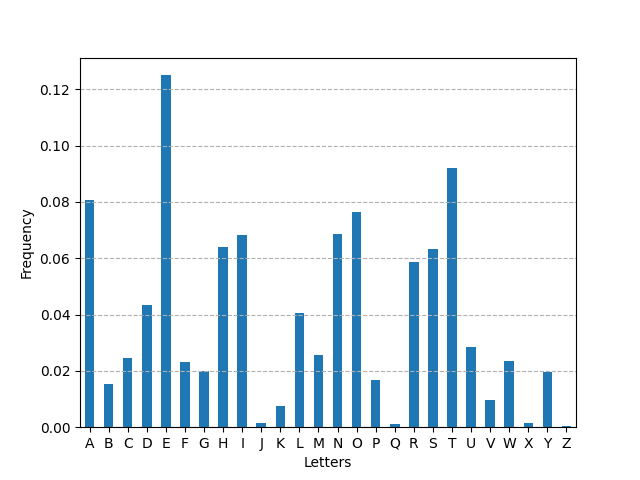
\includegraphics[width=0.48\textwidth]{figures/en.png}
    \caption{English letter frequency}
    \label{fig:en_freq}
\end{figure}
\begin{figure}[H]
    \centering
    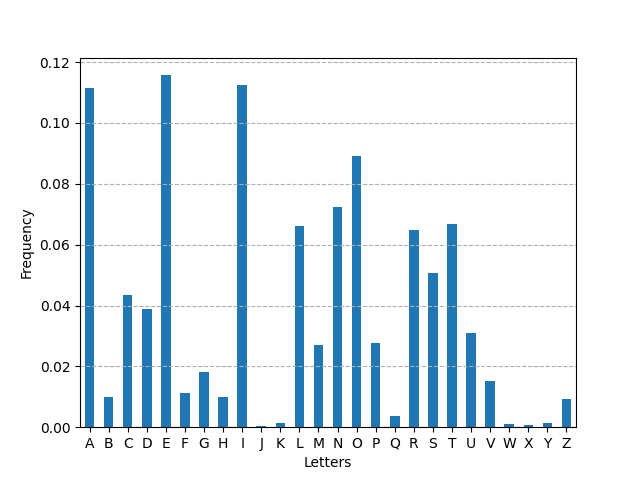
\includegraphics[width=0.48\textwidth]{figures/it.png}
    \caption{Italian letter frequency}
    \label{fig:it_freq}
\end{figure}
\begin{figure}[H]
    \centering
    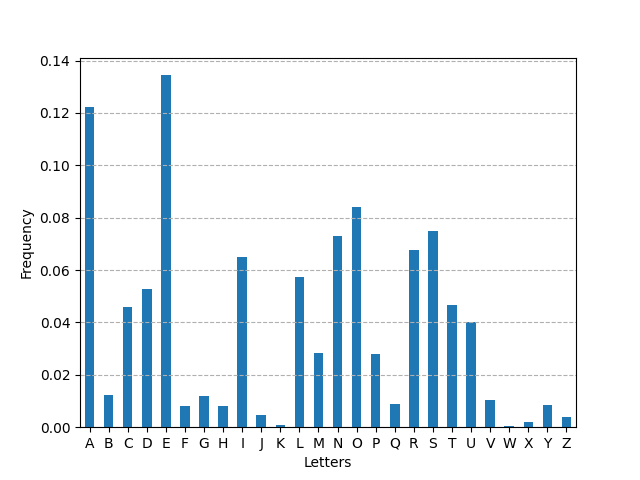
\includegraphics[width=0.48\textwidth]{figures/es.png}
    \caption{Spanish letter frequency}
    \label{fig:es_freq}
\end{figure}

\begin{table}[H]
    \centering
    \begin{tabular}{|c|l|}
        \hline
        Test ID & Arguments \\
        \hline
        0 & \makecell[l]{-i english.txt \\ -r 1} \\        
        \hline
        1 & \makecell[l]{-i english.txt \\ -r 2} \\        
        \hline
        2 & \makecell[l]{-i english.txt \\ -r 4} \\        
        \hline
        3 & \makecell[l]{-i english.txt \\ -r 8} \\        
        \hline
        4 & \makecell[l]{-i english.txt \\ -r 1 \\ --no-combiner} \\        
        \hline
        5 & \makecell[l]{-i english.txt \\ -r 1 \\ --no-in-mapper-combiner} \\        
        \hline
        6 & \makecell[l]{-i english.txt \\ -r 1 \\ --no-in-mapper-combiner \\ --no-combiner} \\        
        \hline
        7 & \makecell[l]{-i english.txt \\ -r 4 \\ --no-combiner} \\        
        \hline
        8 & \makecell[l]{-i english.txt \\ -r 4 \\ --no-in-mapper-combiner} \\        
        \hline
        9 & \makecell[l]{-i english.txt \\ -r 4 \\ --no-in-mapper-combiner \\ --no-combiner} \\        
        \hline
    \end{tabular}
    \caption{General tests}
    \label{tab:general_tests}
\end{table}
\begin{table}[H]
    \centering
    \begin{tabular}{|c|l|}
        \hline
        Test ID & Arguments \\
        \hline
        10 & \makecell[l]{-i part\_100MB.txt \\ -r 1} \\  
        \hline      
        11 & \makecell[l]{-i part\_200MB.txt \\ -r 1} \\  
        \hline      
        12 & \makecell[l]{-i part\_300MB.txt \\ -r 1} \\        
        \hline
        13 & \makecell[l]{-i part\_400MB.txt \\ -r 1} \\        
        \hline
        14 & \makecell[l]{-i part\_500MB.txt \\ -r 1} \\        
        \hline
        15 & \makecell[l]{-i part\_600MB.txt \\ -r 1} \\        
        \hline
        16 & \makecell[l]{-i part\_700MB.txt \\ -r 1} \\        
        \hline
        17 & \makecell[l]{-i part\_800MB.txt \\ -r 1} \\        
        \hline
        18 & \makecell[l]{-i part\_900MB.txt \\ -r 1} \\        
        \hline
        19 & \makecell[l]{-i part\_1000MB.txt \\ -r 1} \\        
        \hline
        20 & \makecell[l]{-i part\_1100MB.txt \\ -r 1} \\            
        \hline
    \end{tabular}
    \caption{Input split tests}
    \label{tab:input_split_tests}
\end{table}

\end{multicols}
\begin{figure}[H]
    \centering
    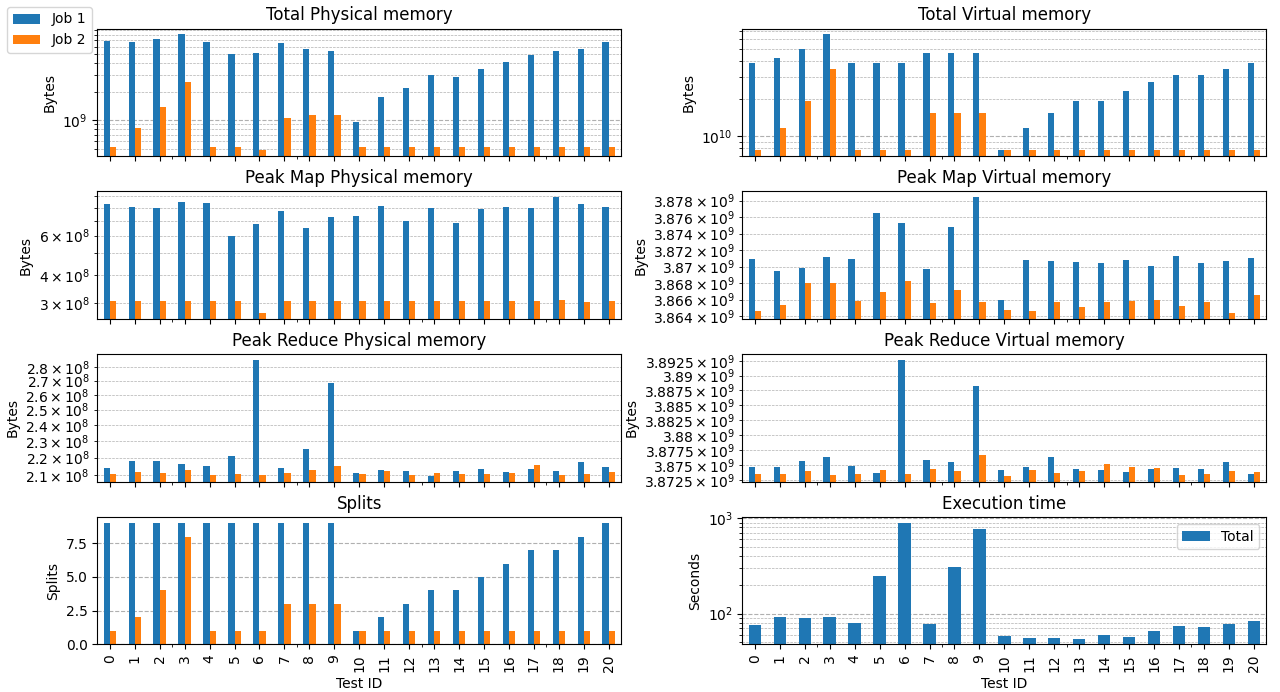
\includegraphics[width=1\textwidth]{figures/experiments.png}
    \caption{Tests results, the x-axis represents the test ID.}
    \label{fig:tests_graph}
\end{figure}
\begin{multicols}{2}
\section{Conclusions}
\end{multicols}

\end{document}